\documentclass[tikz,border=10pt]{standalone}
\usetikzlibrary{positioning}
\usepackage{tkz-graph}
\usepackage{rotating}
\usetikzlibrary{arrows}
\usetikzlibrary{arrows.meta}

\begin{document}
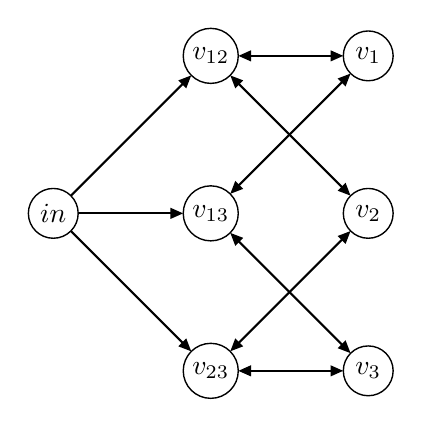
\begin{tikzpicture}
\tikzset{LabelStyle/.style= {circle,inner sep=1pt,minimum size=1pt, orange, text=black}}
\Vertex[x=0 , y=0,L=$in$ ] {in}
\Vertex[x=2 , y=2,L=$v_{12}$] {v12}
\Vertex[x=2 , y=0,L=$v_{13}$ ]  {v13}
\Vertex[x=2 , y	=-2, L=$v_{23}$ ] {v23}
\Vertex[x=4 , y=2, L=$v_{1}$ ] {v1}
\Vertex[x=4 , y=0, L=$v_{2}$ ] {v2}
\Vertex[x=4 , y=-2, L=$v_{3}$ ] {v3}
\Edges[style={-{Triangle[angle=45:5pt]}}](in,v12)
\Edges[style={-{Triangle[angle=45:5pt]}}](in,v13)
\Edges[style={-{Triangle[angle=45:5pt]}}](in,v23)
\Edges[style={{Triangle[angle=45:5pt]}-{Triangle[angle=45:5pt]}}](v13,v1)
\Edges[style={{Triangle[angle=45:5pt]}-{Triangle[angle=45:5pt]}}](v13,v3)
\Edges[style={{Triangle[angle=45:5pt]}-{Triangle[angle=45:5pt]}}](v1,v12)
\Edges[style={{Triangle[angle=45:5pt]}-{Triangle[angle=45:5pt]}}](v2,v23)
\Edges[style={{Triangle[angle=45:5pt]}-{Triangle[angle=45:5pt]}}](v12,v2)
\Edges[style={{Triangle[angle=45:5pt]}-{Triangle[angle=45:5pt]}}](v23,v3)
\end{tikzpicture}
\end{document}
%\tikzset{VertexStyle/.style = {shape = circle, fill = green!20, draw}}
%\tikzset{VertexStyle/.style = {shape = circle, fill = white, draw}}

\SetUpEdge[style={draw=red,very thick,-{Triangle[angle=45:5pt]}}]
\tikzset{LabelStyle/.style ={draw,fill=blue!20}}
\Edges[label=$3$](00,01)